\documentclass[14pt]{extarticle}

\usepackage{amsmath,mathtools,amsfonts,amsthm,amssymb,hyperref,wasysym,xcolor}
\usepackage{parskip,geometry,latexsym,bookmark,mathtools,float,cancel,tcolorbox}

\newtheorem{defn}{Definition}
\newtheorem{thm}{Theorem}
\newtheorem{claim}{Claim}
\newtheorem{lemma}{Lemma}

\newcommand{\dps}{\displaystyle}
\newcommand{\fbl}{\underline{\hspace{1cm}}\,\,}
\newcommand{\R}{\mathbb{R}}
\newcommand{\Z}{\mathbb{Z}}
\newcommand{\Q}{\mathbb{Q}}
\newcommand{\from}{\leftarrow}
\newcommand{\true}{{\bf t}}
\newcommand{\false}{{\bf c}}
\newcommand{\bic}{\leftrightarrow}
\newcommand{\base}[1]{{\color{cyan}#1}}
\newcommand{\da}{\downarrow}
\newcommand{\fa}{\forall}
\newcommand{\te}{\exists}

\hypersetup{colorlinks,allcolors=blue,linktoc=all}
\geometry{a4paper}
\geometry{margin=0.5in}

\title{Chapter 3 Solutions, Susanna Epp Discrete Math 5th Edition}

\author{https://github.com/spamegg1}

\begin{document}
\maketitle
\tableofcontents

\section{Exercise Set 3.1}

\subsection{Exercise 1}
A menagerie consists of seven brown dogs, two black dogs, six gray cats, ten black cats, five blue birds, six yellow birds, and one black bird. Determine which of the following statements are true and which are false.

\subsubsection{(a)}
There is an animal in the menagerie that is red.

\begin{proof}
False (brown, black, gray, blue, yellow, but no red animals).
\end{proof}

\subsubsection{(b)}
Every animal in the menagerie is a bird or a mammal.

\begin{proof}
True (dogs and cats are mammals, the rest are all birds).
\end{proof}

\subsubsection{(c)}
Every animal in the menagerie is brown or gray or black.

\begin{proof}
False (there are blue and yellow animals).
\end{proof}

\subsubsection{(d)}
There is an animal in the menagerie that is neither a cat nor a dog.

\begin{proof}
True (there are birds).
\end{proof}

\subsubsection{(e)}
No animal in the menagerie is blue.

\begin{proof}
False (there are five blue birds).
\end{proof}

\subsubsection{(f)}
There are in the menagerie a dog, a cat, and a bird that all have the same color.

\begin{proof}
True (black).
\end{proof}

\subsection{Exercise 2}
Indicate which of the following statements are true and which are false. Justify your answers as best as you can.

\subsubsection{(a)}
Every integer is a real number.

\begin{proof}
The statement is true. The integers correspond to certain of the points on a number line, and the real numbers correspond to all the points on the number line.
\end{proof}

\subsubsection{(b)}
0 is a positive real number.

\begin{proof}
The statement is false; 0 is neither positive nor negative.
\end{proof}

\subsubsection{(c)}
For every real number $r$, $-r$ is a negative real number.

\begin{proof}
The statement is false. For instance, let $r = -2$. Then $-r = -(-2) = 2$, which is positive.
\end{proof}

\subsubsection{(d)}
Every real number is an integer.

\begin{proof}
The statement is false. For instance, the number $1/2$ is a real number, but it is not an integer.
\end{proof}

\subsection{Exercise 3}
Let $R(m, n)$ be the predicate “If $m$ is a factor of $n^2$ then $m$ is a factor of $n$,” with domain for both $m$ and $n$ being $\Z$ the set of integers.

\subsubsection{(a)}
Explain why $R(m, n)$ is false if $m = 25$ and $n = 10$.

\begin{proof}
When $m = 25$ and $n = 10$, the statement “$m$ is a factor of $n^2$” is true because $n^2 = 100$ and $100 = 4 \cdot 25$. But the statement “$m$ is a factor of $n$” is false because 10 is not a product of 25 times any integer. Thus the hypothesis of $R(m, n)$ is true and the conclusion is false, so the statement as a whole is false.
\end{proof}

\subsubsection{(b)}
Give values different from those in part (a) for which $R(m, n)$ is false.

\begin{proof}
$m = 9$, $n = 12$. 9 is a factor of $12^2 = 144$ because $144 = 9 \cdot 16$ but 9 is not a factor of 12.
\end{proof}

\subsubsection{(c)}
Explain why $R(m, n)$ is true if $m = 5$ and $n = 10$.

\begin{proof}
When $m = 5$ and $n = 10$, both statements “$m$ is a factor of $n^2$” and “$m$ is a factor of $n$” are true because $n^2 = 100 = 5 \cdot 20$ and $n = 10 = 5 \cdot 2$. Thus both the hypothesis and conclusion of $R(m, n)$ are true, and so the statement as a whole is true.
\end{proof}

\subsubsection{(d)}
Give values different from those in part (c) for which $R(m, n)$ is true.

\begin{proof}
$m = 3$, $n = 6$. $6^2 = 36 = 3 \cdot 12$ and $6 = 3 \cdot 2$.
\end{proof}

\subsection{Exercise 4}
Let $Q(x, y)$ be the predicate “If $x < y$ then $x^2 < y^2$” with domain for both $x$ and $y$ being $\R$ the set of real numbers.

\subsubsection{(a)}
Explain why $Q(x, y)$ is false if $x = -2$ and $y = 1$.

\begin{proof}
$Q(-2, 1)$ is the statement “If $-2 < 1$ then $(-2)^2 < 1^2$.” The hypothesis of this statement is $-2 < 1$, which is true. The conclusion is $(-2)^2 < 1^2$, which is false because $(-2)^2 = 4$ and $1^2 = 1$ and $4 \nless 1$. Thus $Q(-2, 1)$ is a conditional statement with a true hypothesis and a false conclusion. So $Q(-2, 1)$ is false.

\end{proof}

\subsubsection{(b)}
Give values different from those in part (a) for which $Q(x, y)$ is false.

\begin{proof}
$x = -5, y = 2$. $-5 < 2$ is true, but $(-5)^2 = 25 < 4 = 2^2$ is false.
\end{proof}

\subsubsection{(c)}
Explain why $Q(x, y)$ is true if $x = 3$ and $y = 8$.

\begin{proof}
$Q(3, 8)$ is the statement “If $3 < 8$ then $3^2 < 8^2$.”
The hypothesis of this statement is $3 < 8$, which is true. The conclusion is $3^2 < 8^2$, which is also true because $3^2 = 9$ and $8^2 = 64$ and $9 < 64$. Thus $Q(3, 8)$ is a conditional statement with a true hypothesis and a true conclusion. So $Q(3, 8)$ is true.
\end{proof}

\subsubsection{(d)}
Give values different from those in part (c) for which $Q(x, y)$ is true.

\begin{proof}
$x = 1, y = 2$. $1 < 2$ is true and $1^2 = 1 < 4 = 2^2$ is true.
\end{proof}

\subsection{Exercise 5}
Find the truth set of each predicate.

\subsubsection{(a)}
Predicate: $6/d$ is an integer, domain: $\Z$

\begin{proof}
The truth set is the set of all integers $d$ such that $6/d$ is an integer, so the truth set is $\{-6, -3, -2, -1, 1, 2, 3, 6\}$.

\end{proof}

\subsubsection{(b)}
Predicate: $6/d$ is an integer, domain: $\Z^+$

\begin{proof}
We take only the positive numbers from the answer in part (a): $\{1, 2, 3, 6\}$.
\end{proof}

\subsubsection{(c)}
Predicate: $1 \leq x^2 \leq 4$, domain: $\R$

\begin{proof}
The truth set is the set of all real numbers x with the property that $1 \leq x^2 \leq 4$, so the truth set is $\{x \in \R \,\, | \,\, -2 \leq x \leq -1 \text{ or } 1 \leq x \leq 2\}$. In other words, the truth set is the set of all real numbers between $-2$ and $-1$ inclusive together with those between 1 and 2 inclusive.
\end{proof}

\subsubsection{(d)}
Predicate: $1 \leq x^2 \leq 4$, domain: $\Z$

\begin{proof}
The truth set is $\{-2, -1, 0, 1, 2\}$.
\end{proof}

\subsection{Exercise 6}
Let $B(x)$ be “$-10 < x < 10$.” Find the truth set of $B(x)$ for each of the following domains.

\subsubsection{(a)}
$\Z$

\begin{proof}
$\{-9, -8, -7, -6, -5, -4, -3, -2, -1, 0, 1, 2, 3, 4, 5, 6, 7, 8, 9\}$
\end{proof}

\subsubsection{(b)}
$\Z^+$
 
\begin{proof}
$\{1, 2, 3, 4, 5, 6, 7, 8, 9\}$
\end{proof}

\subsubsection{(c)}
The set of all even integers

\begin{proof}
$\{-8, -6, -4, -2, 0, 2, 4, 6, 8\}$
\end{proof}

\subsection{Exercise 7}
Let $S$ be the set of all strings of length 3 consisting of $a$’s, $b$’s, and $c$’s. List all the strings in $S$ that satisfy the following conditions:

1. Every string in $S$ begins with $b$.

2. No string in $S$ has more than one $c$.

\begin{proof}
$baa, bab, bac, bba, bbb, bbc, bca, bcb$
\end{proof}

\subsection{Exercise 8}
Let $T$ be the set of all strings of length 3 consisting of 0’s and 1’s. List all the strings in $T$ that satisfy the following conditions:

1. For every string $s$ in $T$, the second character of $s$ is 1 or the first two characters of $s$ are the same.

2. No string in $T$ has all three characters the same.

\begin{proof}
By property 1, any string in $T$ must have one of the forms $x1y$, $00x$ or $11x$.

The possibilities are: for $x1y$: 010, 011, 110, 111; for $00x$: 000, 001; for $11x$: 110, 111.

By property 2 we can eliminate 000 and 111.

So $T = \{010, 011, 110, 001\}$.
\end{proof}

{\bf \color{cyan} Find counterexamples to show that the statements in 9–12 are false.}

\subsection{Exercise 9}
$\fa x \in \R, x \geq 1/x$

\begin{proof}
{\underline Counterexample}: Let $x = 1/2$. Then $1/x = 1/(1/2) = 2$, and $1/2 \ngeq 2$. {\it (This is one counterexample among many.)}
\end{proof}

\subsection{Exercise 10}
$\fa a \in \Z, (a-1)/a$ is not an integer.

\begin{proof}
{\underline Counterexample}: $a = -1$. Then $(a-1)/a = (-1-1)/(-1) = 2$ is an integer. (The only other counterexample is $a = 1$.)
\end{proof}

\subsection{Exercise 11}
$\fa$ positive integers $m$ and $n$, $m \cdot n \geq m + n$.

\begin{proof}
{\underline Counterexample}: Let $m = 1$ and $n = 1$. Then $m\cdot n = 1\cdot 1 = 1$ and $m + n = 1 + 1 = 2$. But $1 \neq 2$, and so $m\cdot n \neq m + n$. {\it (This is one counterexample among many.)}
\end{proof}

\subsection{Exercise 12}
$\fa$ real numbers $x, y$, $\sqrt{x + y} = \sqrt{x} + \sqrt{y}$.

\begin{proof}
{\underline Counterexample}: $x = y = 4$. Then $\sqrt{x + y} = \sqrt{4 + 4} = \sqrt{8} \approx 2.82$ butt $\sqrt{x} + \sqrt{y} = \sqrt{4} + \sqrt{4} = 2 + 2 = 4 \neq 2.82$. {\it (This is one counterexample among many.)}
\end{proof}

\subsection{Exercise 13}
Consider the following statement: $\fa$ basketball player $x$, $x$ is tall.

Which of the following are equivalent ways of expressing this statement?

\subsubsection{(a)}
Every basketball player is tall.

\begin{proof}
This is equivalent. 

We can think of it as follows: the domain $D$ is the set of all people, so it says: ``for all people $x$, if $x$ is a basketball player, then $x$ is tall.''

In other words: $\fa$ people $x$, (BasketballPlayer$(x) \to$ Tall$(x)$).
\end{proof}

\subsubsection{(b)}
Among all the basketball players, some are tall.

\begin{proof}
This is not equivalent. This is making an existential statement: there exists a person who is a basketball player and who is tall. $\te$ person $x$(BasketballPlayer$(x) \wedge$ Tall$(x))$
\end{proof}

\subsubsection{(c)}
Some of all the tall people are basketball players.

\begin{proof}
This is not equivalent. This is making an existential statement: $\te$ person $x$ such that Tall($x$) and BasketballPlayer($x$).
\end{proof}

\subsubsection{(d)}
Anyone who is tall is a basketball player.

\begin{proof}
This is not equivalent. It states the converse of the original statement: $\fa$ people $x$, if Tall($x$) then BasketballPlayer($x$).
\end{proof}

\subsubsection{(e)}
All people who are basketball players are tall.

\begin{proof}
This is equivalent. It says: $\fa$ people $x$, if BasketballPlayer($x$) then Tall($x$).
\end{proof}

\subsubsection{(f)}
Anyone who is a basketball player is a tall person.

\begin{proof}
This is equivalent, same as (e).
\end{proof}

\subsection{Exercise 14}
Consider the following statement: $\te x \in \R$ such that $x^2 = 2$.

Which of the following are equivalent ways of expressing this statement?

\subsubsection{(a)}
The square of each real number is 2.

\begin{proof}
This is not equivalent. This is a universal statement: $\fa x \in \R(x^2 = 2)$. The word ``each'' here means ``every'', which is a universal quantifier.
\end{proof}

\subsubsection{(b)}
Some real numbers have square 2.

\begin{proof}
This is equivalent. ``Some: is an existential quantifier. So it says $\te x \in \R (x^2 = 2)$.
\end{proof}

\subsubsection{(c)}
The number $x$ has square 2, for some real number $x$.

\begin{proof}
This is equivalent like (b), just written differently (two halves of the sentence are swapped). ``Some'' is an existential quantifier.
\end{proof}

\subsubsection{(d)}
If $x$ is a real number, then $x^2 = 2$.

\begin{proof}
This is not equivalent. This is making a universal statement about all real numbers: ``if $x$ is a real number, then ...'' So it is equivalent to $\fa x \in \R (x^2 = 2)$.
\end{proof}

\subsubsection{(e)}
Some real number has square 2.

\begin{proof}
This is equivalent, just like (b) and (c) but written differently.
\end{proof}

\subsubsection{(f)}
There is at least one real number whose square is 2.

\begin{proof}
This is equivalent. ``There is at least one'' is an existential quantifier.
\end{proof}

\subsection{Exercise 15}
Rewrite the following statements informally in at least two different ways without using variables or quantifiers.

\subsubsection{(a)}
$\fa$ rectangle $x$, $x$ is a quadrilateral.

\begin{proof}
Every rectangle is a quadrilateral.

All rectangles are quadrilaterals.
\end{proof}

\subsubsection{(b)}
$\te$ a set $A$ such that $A$ has 16 subsets.

\begin{proof}
At least one set has 16 subsets.

Some set has 16 subsets.
\end{proof}

\subsection{Exercise 16}
Rewrite each of the following statements in the form “$\fa \fbl x, \fbl$.”

\subsubsection{(a)}
All dinosaurs are extinct.

\begin{proof}
$\fa$ dinosaur $x$, $x$ is extinct.
\end{proof}

\subsubsection{(b)}
Every real number is positive, negative, or zero.

\begin{proof}
$\fa$ real number $x$, $x$ is positive, negative or zero.
\end{proof}

\subsubsection{(c)}
No irrational numbers are integers.

\begin{proof}
$\fa$ irrational number $x$, $x$ is not an integer.
\end{proof}

\subsubsection{(d)}
No logicians are lazy.

\begin{proof}
$\fa$ logician $x$, $x$ is not lazy.
\end{proof}

\subsubsection{(e)}
The number 2,147,581,953 is not equal to the square of any integer.

\begin{proof}
$\fa$ integer $x$, $x^2$ does not equal 2,147,581,953.
\end{proof}

\subsubsection{(f)}
The number $-1$ is not equal to the square of any real number.

\begin{proof}
$\fa$ real number $x$, $x^2$ does not equal $-1$.
\end{proof}

\subsection{Exercise 17}
Rewrite each of the following in the form “$\te \fbl x$ such that \fbl.”

\subsubsection{(a)}
Some exercises have answers.

\begin{proof}
$\te$ exercise $x$ such that $x$ has an answer.
\end{proof}

\subsubsection{(b)}
Some real numbers are rational.

\begin{proof}
$\te$ real number $x$ such that $x$ is rational.
\end{proof}

\subsection{Exercise 18}
Let $D$ be the set of all students at your school, and let $M(s)$ be “$s$ is a math major,” let $C(s)$ be “$s$ is a computer science student,” and let $E(s)$ be “$s$ is an engineering student.” Express each of the following statements using quantifiers, variables, and the predicates $M(s), C(s)$, and $E(s)$.

\subsubsection{(a)}
There is an engineering student who is a math major.

\begin{proof}
$\te s \in D$ such that $E(s)$ and $M(s)$. (Or: $\te s \in D$ such that $E(s) \wedge M(s)$.)
\end{proof}

\subsubsection{(b)}
Every computer science student is an engineering student.

\begin{proof}
$\fa s \in D$, if $C(s)$ then $E(s)$. (Or: $\fa s \in D, C(s) \to E(s)$.)
\end{proof}

\subsubsection{(c)}
No computer science students are engineering students.

\begin{proof}
$\fa s \in D$, $C(s) \to \sim E(s)$.
\end{proof}

\subsubsection{(d)}
Some computer science students are also math majors.

\begin{proof}
$\te s \in D$ such that $C(s) \wedge M(s)$.
\end{proof}

\subsubsection{(e)}
Some computer science students are engineering students and some are not.

\begin{proof}
$(\te s \in D$ such that $C(s) \wedge E(s)$) $\wedge$ $(\te s \in D$ such that $C(s) \wedge \sim E(s))$.
\end{proof}

\subsection{Exercise 19}
Consider the following statement: $\fa$ integer $n$, if $n^2$ is even then $n$ is even.

Which of the following are equivalent ways of expressing this statement?

\subsubsection{(a)}
All integers have even squares and are even.

\begin{proof}
This is not equivalent. This says: $\fa$ integer $n$, $n^2$ is even and $n$ is even.
\end{proof}

\subsubsection{(b)}
Given any integer whose square is even, that integer is itself even.

\begin{proof}
This is equivalent. This says: $\fa$ integer $n$, $n^2$ is even and $n$ is even.
\end{proof}

\subsubsection{(c)}
For all integers, there are some whose square is even.

\begin{proof}
This is not equivalent. This says: $\fa$ integer $n$, $n^2$ is even and $n$ is even.
\end{proof}

\subsubsection{(d)}
Any integer with an even square is even.

\begin{proof}
This is equivalent. This says: $\fa$ integer $n$, $n^2$ is even and $n$ is even.
\end{proof}

\subsubsection{(e)}
If the square of an integer is even, then that integer is even.

\begin{proof}
This is equivalent. This says: $\fa$ integer $n$, $n^2$ is even and $n$ is even.
\end{proof}

\subsubsection{(f)}
All even integers have even squares.

\begin{proof}
This is not equivalent. This says: $\fa$ integer $n$, if $n$ is even then $n^2$ is even. (converse)
\end{proof}

\subsection{Exercise 20}
Rewrite the following statement informally in at least two different ways without using variables or the symbol $\fa$ or the words “for all.”

$\fa$ real numbers $x$, if $x$ is positive then the square root of $x$ is positive.

\begin{proof}
The square root of a positive real number is positive.

If a real number is positive, then its square root is positive.
\end{proof}

\subsection{Exercise 21}
Rewrite the following statements so that the quantifier trails the rest of the sentence.

\subsubsection{(a)}
For any graph $G$, the total degree of $G$ is even.

\begin{proof}
The total degree of $G$ is even, for any graph $G$.
\end{proof}

\subsubsection{(b)}
For any isosceles triangle $T$, the base angles of $T$ are equal.

\begin{proof}
The base angles of $T$ are equal, for any isosceles triangle $T$.
\end{proof}

\subsubsection{(c)}
There exists a prime number $p$ such that $p$ is even.

\begin{proof}
$p$ is even, for some a prime number $p$.
\end{proof}

\subsubsection{(d)}
There exists a continuous function $f$ such that $f$ is not differentiable.

\begin{proof}
$f$ is not differentiable, for some continuous function $f$.
\end{proof}

\subsection{Exercise 22}
Rewrite each of the following statements in the form “$\fa \fbl x$, if \fbl then \fbl.”

\subsubsection{(a)}
All Java programs have at least 5 lines.

\begin{proof}
$\fa x$, if $x$ is a Java program, then $x$ has at least 5 lines.
\end{proof}

\subsubsection{(b)}
Any valid argument with true premises has a true conclusion.

\begin{proof}
$\fa$ argument $x$, if $x$ is valid with true premises, then $x$ has a true conclusion.
\end{proof}

\subsection{Exercise 23}
Rewrite each of the following statements in the two forms “$\fa x$, if \fbl then \fbl” and “$\fa x$, \fbl” (without an if-then).

\subsubsection{(a)}
All equilateral triangles are isosceles.

\begin{proof}
$\fa x$ if $x$ is an equilateral triangle, then $x$ is isosceles.

$\fa$ equilateral triangles $x$, $x$ is isosceles.
\end{proof}

\subsubsection{(b)}
Every computer science student needs to take data structures.

\begin{proof}

\end{proof}

\subsection{Exercise 24}
Rewrite the following statements in the two forms “$\te \fbl x$ such that \fbl” and “$\te x$ such that \fbl and \fbl.”

\subsubsection{(a)}
Some hatters are mad.

\begin{proof}
$\te$ a hatter $x$ such that $x$ is mad.

$\te x$ such that $x$ is a hatter and $x$ is mad.
\end{proof}

\subsubsection{(b)}
Some questions are easy.

\begin{proof}
$\te$ a question $x$ such that $x$ is easy.

$\te x$ such that $x$ is a question and $x$ is easy.
\end{proof}

\subsection{Exercise 25}
The statement “The square of any rational number is rational” can be rewritten formally as “For all rational numbers $x$, $x^2$ is rational” or as “For all $x$, if $x$ is rational then $x^2$ is rational.” Rewrite each of the following statements in the two forms “$\fa \fbl x$, \fbl” and “$\fa x$, if \fbl, then \fbl” or in the two forms “$\fa \fbl x$ and $y$, ”\fbl and “$\fa x$ and $y$, if \fbl, then \fbl.”

\subsubsection{(a)}
The reciprocal of any nonzero fraction is a fraction.

\begin{proof}
$\fa$ nonzero fraction $x$, the reciprocal of $x$ is a fraction.

$\fa x$, if $x$ is a nonzero fraction then the reciprocal of $x$ is a fraction.
\end{proof}

\subsubsection{(b)}
The derivative of any polynomial function is a polynomial function.

\begin{proof}
$\fa$ polynomial function $x$, the derivative of $x$ is a polynomial function. 

$\fa x$, if $x$ is a polynomial function, then the derivative of $x$ is a polynomial function.
\end{proof}

\subsubsection{(c)}
The sum of the angles of any triangle is 180°.

\begin{proof}
$\fa$ triangle $x$, the sum of the angles of $x$ is 180°. 

$\fa x$, if $x$ is a triangle then the sum of the angles of $x$ is 180°.
\end{proof}

\subsubsection{(d)}
The negative of any irrational number is irrational.

\begin{proof}
$\fa$ irrational number $x$, $-x$ is irrational. 

$\fa x$, if $x$ is an irrational number, then $-x$ is irrational.
\end{proof}

\subsubsection{(e)}
The sum of any two even integers is even.

\begin{proof}
$\fa$ even integers $x$ and $y$, the sum of $x$ and $y$ is even.

$\fa x$ and $y$, if $x$ and $y$ are even integers then the sum of $x$ and $y$ is even.
\end{proof}

\subsubsection{(f)}
The product of any two fractions is a fraction.

\begin{proof}
$\fa$ fractions $x$ and $y$, the product of $x$ and $y$ is a fraction.

$\fa x$ and $y$, if $x$ and $y$ are fractions then the product of $x$ and $y$ is a fraction.
\end{proof}

\subsection{Exercise 26}
Consider the statement “All integers are rational numbers but some rational numbers are not integers.”

\subsubsection{(a)}
Write this statement in the form “$\fa x$, if \fbl then \fbl, but $\te \fbl x$ such that \fbl.”

\begin{proof}
$\fa x$, if $x$ is an integer then $x$ is a rational number, but $\te$ rational number $x$ such that $x$ is not an integer.
\end{proof}

\subsubsection{(b)}
Let Ratl($x$) be “$x$ is a rational number” and Int($x$) be “$x$ is an integer.” Write the given statement formally using only the symbols Ratl($x$), Int($x$), $\fa, \te, \wedge, \vee, \sim,$ and $\to$.

\begin{proof}
$\fa x$ (Int($x$) $\to$ Ratl($x$)) $\wedge$ $\te x$ (Ratl($x$) $\wedge \sim$ Int($x$))
\end{proof}

\subsection{Exercise 27}
\begin{figure}[ht!]
\centering
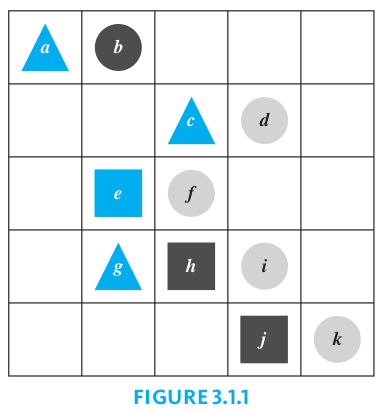
\includegraphics[scale=0.4]{../images/3.1.1.png}
\end{figure}

Refer to Figure 3.1.1 of Tarski’s world given in Example 3.1.13. Let Above($x, y$) mean that $x$ is above $y$ (but possibly in a different column). Determine the truth or falsity of each of the following statements. Give reasons for your answers.

\subsubsection{(a)}
$\fa u$, Circle($u$) $\to$ Gray($u$).

\begin{proof}
False. Figure $b$ is a circle that is not gray.
\end{proof}

\subsubsection{(b)}
$\fa u$, Gray($u$) $\to$ Circle($u$).

\begin{proof}
True. All the gray figures are circles.
\end{proof}

\subsubsection{(c)}
$\te y$ such that Square($y$) $\wedge$ Above($y, d$).

\begin{proof}
False. There are no squares above $d$.
\end{proof}

\subsubsection{(d)}
$\te z$ such that Triangle($z$) $\wedge$ Above($f, z$).

\begin{proof}
True. $z = g$ satisfies this statement.
\end{proof}

{\bf \color{cyan} In $28-30$, rewrite each statement without using quantifiers or variables. Indicate which are true and which are false, and justify your answers as best as you can.}

\subsection{Exercise 28}
Let the domain of $x$ be the set $D$ of objects discussed in mathematics courses, and let Real($x$) be “$x$ is a real number,” Pos($x$) be “$x$ is a positive real number,” Neg($x$) be “$x$ is a negative real number,” and Int($x$) be “$x$ is an integer.”

\subsubsection{(a)}
Pos(0)

\begin{proof}
0 is a positive real number. True.
\end{proof}

\subsubsection{(b)}
$\fa x$, Real($x$) $\wedge$ Neg($x$) $\to$ Pos($-x$)

\begin{proof}
{\it One answer among many}: If a real number is negative, then when its opposite is computed, the result is a positive real number.

This statement is true because for each real number $x$, $-(-|x|) = |x|$ (and any negative real number can be represented as $-|x|$, for some real number $x$).
\end{proof}

\subsubsection{(c)}
$\fa x$, Int($x$) $\to$ Real$(x)$

\begin{proof}
Every integer is a real number. True.
\end{proof}

\subsubsection{(d)}
$\te x$ such that, Real($x$) $\wedge$ $\sim$ Int($x$) 

\begin{proof}
{\it One answer among many}: There is a real number that is not an integer. This statement is true. For instance, $1/2$ is a real number that is not an integer.
\end{proof}

\subsection{Exercise 29}
Let the domain of $x$ be the set of geometric figures in the plane, and let Square($x$) be “$x$ is a square” and Rect($x$) be “$x$ is a rectangle.”

\subsubsection{(a)}
$\te x$ such that Rect($x$) $\wedge$ Square($x$)

\begin{proof}
There is a rectangle that is a square. True.
\end{proof}

\subsubsection{(b)}
$\te x$ such that Rect($x$) $\wedge \sim$ Square($x$)

\begin{proof}
There is a rectangle that is not a square. True.
\end{proof}

\subsubsection{(c)}
$\fa x$, Square($x$) $\to$ Rect($x$)

\begin{proof}
Every square is a rectangle. True.
\end{proof}

\subsection{Exercise 30}
Let the domain of $x$ be $\Z$, the set of integers, and let Odd($x$) be “$x$ is odd,” Prime($x$) be “$x$ is prime,” and Square($x$) be “$x$ is a perfect square.” (An integer $n$ is said to be a perfect square if, and only if, it equals the square of some integer. For example, 25 is a perfect square because $25 = 5^2$.)

\subsubsection{(a)}
$\te x$ such that Prime($x$) $\wedge\sim$Odd($x$)

\begin{proof}
There is a prime number that is not odd. True: 2.
\end{proof}

\subsubsection{(b)}
$\fa x$, Prime($x$) $\to$ $\sim$Square($x$)

\begin{proof}
{\it One answer among many}: If an integer is prime, then it is not a perfect square.

This statement is true because a prime number is an integer greater than 1 that is not a product of two smaller positive integers. So a prime number cannot be a perfect square because if it were, it would be a product of two smaller positive integers.
\end{proof}

\subsubsection{(c)}
$\te x$ such that Odd($x$) $\wedge$ Square($x$)

\begin{proof}
There is an odd integer that is a perfect square. True: 9.
\end{proof}

\subsection{Exercise 31}
In any mathematics or computer science text other than this book, find an example of a statement that is universal but is implicitly quantified. Copy the statement as it appears and rewrite it making the quantification explicit. Give a complete citation for your example, including title, author, publisher, year, and page number.

\begin{proof}
{\it Hint:} Your answer should have the appearance shown in
the following made-up example:

{\it Statement:} “If a function is differentiable, then it is continuous.”

{\it Formal version:} $\fa$ function $f$, if $f$ is differentiable, then $f$ is continuous.

{\it Citation: Calculus} by D. R. Mathematician, Best Publishing Company, 2019, page 263.
\end{proof}

\subsection{Exercise 32}
Let $\R$ be the domain of the predicate variable $x$. Which of the following are true and which are false? Give counter examples for the statements that are false.

\subsubsection{(a)}
$x > 2 \implies x > 1$

\begin{proof}
True: Any real number that is greater than 2 is greater than 1.
\end{proof}

\subsubsection{(b)}
$x > 2 \implies x^2 > 4$

\begin{proof}
True.
\end{proof}

\subsubsection{(c)}
$x^2 > 4 \implies x > 2$

\begin{proof}
False: $(-3)^2 > 4$ but $-3 \ngtr 2$.
\end{proof}

\subsubsection{(d)}
$x^2 > 4 \iff |x| > 2$

\begin{proof}
True.
\end{proof}

\subsection{Exercise 33}
Let $\R$ be the domain of the predicate variables $a, b, c$, and $d$. Which of the following are true and which are false? Give counterexamples for the statements that are false.

\subsubsection{(a)}
$a > 0$ and $b > 0 \implies ab > 0$

\begin{proof}
True. Whenever both a and b are positive, so is their product.
\end{proof}

\subsubsection{(b)}
$a < 0$ and $b < 0 \implies ab < 0$

\begin{proof}
False. Let $a = -2$ and $b = -3$. Then $ab = 6$, which is not less than zero.
\end{proof}

\subsubsection{(c)}
$ab = 0 \implies a = 0$ or $b = 0$

\begin{proof}
True.
\end{proof}

\subsubsection{(d)}
$a < b$ and $c < d \implies ac < bd$

\begin{proof}
False. $a = -1$, $b = 1$, $c = -1$, $d = 1$. Then $a < b$ because $-1 < 1$. Similarly $c < d$ is true. But $ac = 1 = bd$ and $1 \nless 1$.
\end{proof}

\section{Exercise Set 3.2}

\subsection{Exercise 1}
Which of the following is a negation for “All discrete mathematics students are athletic”? More than one answer may be correct.

{\it Solution:} Original statement is: $\fa s$ (DiscMath($s$) $\to$ Athletic($s$)). 

Negation is $\sim \fa s$ (DiscMath($s$) $\to$ Athletic($s$)) $\equiv$ $\te s \sim$ (DiscMath($s$) $\to$ Athletic($s$)) $\equiv$ $\te s \sim$ ($\sim$ DiscMath($s$) $\vee$ Athletic($s$)) $\equiv$ $\te s$ (DiscMath($s$) $\wedge \sim$ Athletic($s$)).

Which is: ``There is a student $s$ such that $s$ is a discrete mathematics student AND $s$ is not athletic.''

\subsubsection{(a)}
There is a discrete mathematics student who is nonathletic.

\begin{proof}
Equivalent to the negation.
\end{proof}

\subsubsection{(b)}
All discrete mathematics students are nonathletic.

\begin{proof}
Not equivalent to the negation. This says: $\fa s$ (DiscMath($s$) $\to\sim$ Athletic($s$)).
\end{proof}

\subsubsection{(c)}
There is an athletic person who is not a discrete mathematics student.

\begin{proof}
Not equivalent to the negation. This says: $\te s$ (Athletic($s$) $\wedge \sim$ DiscMath($s$)).
\end{proof}

\subsubsection{(d)}
No discrete mathematics students are athletic.

\begin{proof}
Not equivalent to the negation. This says: $\fa s$ (DiscMath($s$) $\to \sim$ Athletic($s$))
\end{proof}

\subsubsection{(e)}
Some discrete mathematics students are nonathletic.

\begin{proof}
Equivalent to the negation.
\end{proof}

\subsubsection{(f)}
No athletic people are discrete mathematics students.

\begin{proof}
Not equivalent to the negation. This says: $\fa s$ (Athletic($s$) $\to \sim$ DiscMath($s$))
\end{proof}

\subsection{Exercise 2}
Which of the following is a negation for “All dogs are loyal”? More than one answer may be correct.

{\it Solution.} The statement is: $\fa x$ (Dog($x$) $\to$ Loyal($x$)).

The negation is: $\te x$ (Dog($x$) $\wedge \sim$ Loyal($x$)).

\subsubsection{(a)}
All dogs are disloyal.

\begin{proof}
Not equivalent to the negation. This says: $\fa x$ (Dog($x$) $\to\sim$ Loyal($x$)).
\end{proof}

\subsubsection{(b)}
No dogs are loyal.

\begin{proof}
Not equivalent to the negation. This says the same as (a).
\end{proof}

\subsubsection{(c)}
Some dogs are disloyal.

\begin{proof}
Equivalent to the negation.
\end{proof}

\subsubsection{(d)}
Some dogs are loyal.

\begin{proof}
Not equivalent to the negation. This says: $\te x$ (Dog($x$) $\wedge$ Loyal($x$)).
\end{proof}

\subsubsection{(e)}
There is a disloyal animal that is not a dog.

\begin{proof}
Not equivalent to the negation. This says: $\te x$ ($\sim$ Dog($x$) $\wedge\sim$ Loyal($x$)).
\end{proof}

\subsubsection{(f)}
There is a dog that is disloyal.

\begin{proof}
Equivalent to the negation. This says: $\te x$ (Dog($x$) $\wedge\sim$ Loyal($x$)).
\end{proof}

\subsubsection{(g)}
No animals that are not dogs are loyal.

\begin{proof}
Not equivalent to the negation. This says: $\fa x$ ($\sim$ Dog($x$) $\to\sim$ Loyal($x$)).
\end{proof}

\subsubsection{(h)}
Some animals that are not dogs are loyal.

\begin{proof}
Not equivalent to the negation. This says: $\te x$ ($\sim$ Dog($x$) $\wedge$ Loyal($x$)).
\end{proof}

\subsection{Exercise 3}
Write a formal negation for each of the following statements.

\subsubsection{(a)}
$\fa$ string $s$, $s$ has at least one character.

\begin{proof}
$\te$ a string $s$ such that $s$ does not have any characters.

(Or: $\te$ a string $s$ such that $s$ has no characters.)
\end{proof}

\subsubsection{(b)}
$\fa$ computer $c$, $c$ has a CPU.

\begin{proof}
$\te$ computer $c$ such that $c$ does not have a CPU.
\end{proof}

\subsubsection{(c)}
$\te$ a movie $m$ such that $m$ is over 6 hours long.

\begin{proof}
$\fa$ movie $m$, $m$ is less than or equal to 6 hours long.

(Or: $\fa$ movie $m$, $m$ is no more than 6 hours long.)
\end{proof}

\subsubsection{(d)}
$\te$ a band $b$ such that $b$ has won at least 10 Grammy awards.

\begin{proof}
$\fa$ band $b$, $b$ has not won at least 10 Grammy awards.
\end{proof}

{\bf \color{cyan} In $4-6$ there are other correct answers in addition to those shown.}

\subsection{Exercise 4}
Write an informal negation for each of the following statements. Be careful to avoid negations that are ambiguous.

\subsubsection{(a)}
All dogs are friendly.

\begin{proof}
Some dogs are unfriendly. (Or: There is at least one
unfriendly dog.)

\end{proof}

\subsubsection{(b)}
All graphs are connected.

\begin{proof}
Some graphs are not connected.
\end{proof}

\subsubsection{(c)}
Some suspicions were substantiated.

\begin{proof}
All suspicions were unsubstantiated. (Or: No suspicions were substantiated.)
\end{proof}

\subsubsection{(d)}
Some estimates are accurate.

\begin{proof}
All estimates are inaccurate.
\end{proof}

\subsection{Exercise 5}
Write a negation for each of the following statements.

\subsubsection{(a)}
Every valid argument has a true conclusion.

\begin{proof}
There is a valid argument that does not have a true
conclusion. (Or: There is at least one valid argument
that does not have a true conclusion.)
\end{proof}

\subsubsection{(b)}
All real numbers are positive, negative, or zero.

\begin{proof}
Some real numbers are not positive, negative, or zero. (Or: there is a real number that is not positive and is not negative and is not zero.)
\end{proof}

{\bf \color{cyan}Write a negation for each statement in 6 and 7.}

\subsection{Exercise 6}

\subsubsection{(a)}
Sets $A$ and $B$ do not have any points in common.

\begin{proof}
Sets A and B have at least one point in common.
\end{proof}

\subsubsection{(b)}
Towns $P$ and $Q$ are not connected by any road on the map.

\begin{proof}
Towns $P$ and $Q$ are connected by some road on the map.
\end{proof}

\subsection{Exercise 7}

\subsubsection{(a)}
This vertex is not connected to any other vertex in the graph.

\begin{proof}
This vertex is connected to at least one other vertex in the graph. (Or: There is at least one other vertex in the graph to which this vertex is connected.) (Or: This vertex is connected to some other vertex in the graph.)
\end{proof}

\subsubsection{(b)}
This number is not related to any even number.

\begin{proof}
This number is related to some even number.
\end{proof}

\subsection{Exercise 8}
Consider the statement “There are no simple solutions to life’s problems.” Write an informal negation for the statement, and then write the statement formally using quantifiers and variables.

\begin{proof}
Informal: “There is a simple solution to life’s problems.”

Formal: $\te x$ such that $x$ is a simple solution to life's problems.
\end{proof}

{\bf \color{cyan}Write a negation for each statement in 9 and 10.}

\subsection{Exercise 9}
$\fa$ real number $x$, if $x > 3$ then $x^2 > 9$.

\begin{proof}
$\te$ a real number $x$ such that $x > 3$ and $x^2 \leq 9$.
\end{proof}

\subsection{Exercise 10}
$\fa$ computer program $P$, if $P$ compiles without error messages, then $P$ is correct.

\begin{proof}
$\te$ computer program $P$ such that $P$ compiles without error messages and $P$ is not correct.
\end{proof}

{\bf \color{cyan} In each of $11-14$ determine whether the proposed negation is correct. If it is not, write a correct negation.}

\subsection{Exercise 11}
Statement: The sum of any two irrational numbers is irrational.

Proposed negation: The sum of any two irrational numbers is rational.

\begin{proof}
The proposed negation is not correct. The given statement makes a claim about any two irrational numbers and means that no matter what two irrational numbers you might choose, the sum of those numbers will be irrational. For this to be false means that there is at least one pair of irrational numbers whose sum is rational. 

On the other hand, the negation proposed in the exercise (“The sum of any two irrational numbers is rational”) means that given any two irrational numbers, their sum is rational. This is a much stronger statement than the actual negation: The truth of this statement implies the truth of the negation (assuming that there are at least two irrational numbers), but the negation can be true without having this statement be true.

Correct negation: There are at least two irrational numbers whose sum is rational.

Or: The sum of some two irrational numbers is rational.
\end{proof}

\subsection{Exercise 12}
Statement: The product of any irrational number and any rational number is irrational.

Proposed negation: The product of any irrational number and any rational number is rational.

\begin{proof}
The proposed negation is wrong.

Statement (formally): $\fa x \fa y$ (Irrational($x$) $\wedge$ Rational($y$) $\to$ Irrational($x \cdot y$))

Correct negation (formally): $\te x \te y$ (Irrational($x$) $\wedge$ Rational($y$) $\wedge\sim$ Irrational($x \cdot y$))

Proposed negation (formally): $\fa x \fa y$ (Irrational($x$) $\wedge$ Rational($y$) $\to$ Rational($x \cdot y$))

The given statement makes a claim about any pair of numbers, where one number is irrational and the other rational; and means that no matter what two numbers you might choose, the product of those numbers will be irrational. For this to be false means that there is at least one (irrational, rational) pair of numbers whose product is rational. 

On the other hand, the negation proposed in the exercise means that given any (irrational, rational) pair of numbers, their product is rational. This is a much stronger statement than the actual negation: The truth of this statement implies the truth of the negation, but the negation can be true without having this statement be true.

Correct negation: There is an irrational number and a rational number, whose product is rational.
\end{proof}

\subsection{Exercise 13}
Statement: For every integer $n$, if $n^2$ is even then $n$ is even.

Proposed negation: For every integer $n$, if $n^2$ is even then $n$ is not even.

\begin{proof}
The proposed negation is not correct. There are two mistakes: The negation of a “for every” statement is not a “for every” statement; and the negation of an if-then statement is not an if-then statement. 

Correct negation: There exists an integer $n$ such that $n^2$ is even and $n$ is not even.
\end{proof}

\subsection{Exercise 14}
Statement: For all real numbers $x_1$ and $x_2$, if $x_1^2 = x_2^2$ then $x_1 = x_2$.

Proposed negation: For all real numbers $x_1$ and $x_2$, if $x_1^2 = x_2^2$ then $x1 \neq x2$.

\begin{proof}
The proposed negation is wrong. The issue is the same as in Exercise 12. The negation only requires one pair of numbers to fail to satisfy the if-then statement; the proposed negation says that all pairs fail to satisfy the if-then statement.

Correct negation: There exist real numbers $x_1$ and $x_2$ such that $x_1^2 = x_2^2$ but $x_1 \neq x_2$.
\end{proof}

\subsection{Exercise 15}
Let $D = \{-48, -14, -8, 0, 1, 3, 16, 23, 26, 32, 36\}$.
Determine which of the following statements are true and which are false. Provide counterexamples for the statements that are false.

\subsubsection{(a)}
$\fa x \in D$, if $x$ is odd then $x > 0$.

\begin{proof}
True: All the odd numbers in $D$ are positive.
\end{proof}

\subsubsection{(b)}
$\fa x \in D$, if $x$ is less than 0 then $x$ is even.

\begin{proof}
True. All the negative numbers in $D$ are even.
\end{proof}

\subsubsection{(c)}
$\fa x \in D$, if $x$ is even then $x \leq 0$.

\begin{proof}
False: $x = 16, x = 26, x = 32$, and $x = 36$ are all
counterexamples.
\end{proof}

\subsubsection{(d)}
$\fa x \in D$, if the ones digit of $x$ is 2, then the tens digit is 3 or 4.

\begin{proof}
True: the only number in $D$ with the ones digit 2 is 32.
\end{proof}

\subsubsection{(e)}
$\fa x \in D$, if the ones digit of $x$ is 6, then the tens digit is 1 or 2.

\begin{proof}
False: $x = 36$ is a counterexample.
\end{proof}

{\bf \color{cyan} In $16-23$, write a negation for each statement.}

\subsection{Exercise 16}
$\fa$ real number $x$, if $x^2 \geq 1$ then $x > 0$.

\begin{proof}
$\te$ a real number $x$ such that $x^2 \geq 1$ and $x \ngtr 0$. 

In other words, $\te$ a real number $x$ such that $x^2 \geq 1$ and $x \leq 0$.
\end{proof}

\subsection{Exercise 17}
$\fa$ integer $d$, if $6 / d$ is an integer then $d = 3$.

\begin{proof}
$\te$ integer $d$ such that $6 / d$ is an integer but $d \neq 3$.
\end{proof}

\subsection{Exercise 18}
$\fa x \in \R$, if $x(x + 1) > 0$ then $x > 0$ or $x < -1$.

\begin{proof}
$\te x \in \R$ such that $x(x + 1) > 0$ and both $x \leq 0$ and $x \geq -1$.
\end{proof}

\subsection{Exercise 19}
$\fa n \in \Z$, if $n$ is prime then $n$ is odd or $n = 2$.

\begin{proof}
$\te n \in \Z$ such that $n$ is prime and both $n$ is even and $n \neq 2$.
\end{proof}

\subsection{Exercise 20}
$\fa$ integers $a, b$, and $c$, if $a - b$ is even and $b - c$ is even, then $a - c$ is even.

\begin{proof}
$\te$ integers $a, b$ and $c$ such that $a - b$ is even and $b - c$ is even, and $a - c$ is not even.
\end{proof}

\subsection{Exercise 21}
$\fa$ integer $n$, if $n$ is divisible by 6, then $n$ is divisible by 2 and $n$ is divisible by 3.

\begin{proof}
$\te$ an integer $n$ such that $n$ is divisible by 6, and either $n$ is not divisible by 2 or $n$ is not divisible by 3.
\end{proof}

\subsection{Exercise 22}
If the square of an integer is odd, then the integer is odd.

\begin{proof}
There is an integer with the property that the square of the integer is odd but the integer itself is not odd. 

(Or: At least one integer has an odd square but is not itself odd.)
\end{proof}

\subsection{Exercise 23}
If a function is differentiable then it is continuous.

\begin{proof}
$\te$ a function that is differentiable and is not continuous.
\end{proof}

\subsection{Exercise 24}
Rewrite the statements in each pair in if-then form and indicate the logical relationship between them.

\subsubsection{(a)}
All the children in Tom’s family are female. 

All the females in Tom’s family are children.

\begin{proof}
If a person is a child in Tom’s family, then the person is female.

If a person is a female in Tom’s family, then the person is a child.

The second statement is the converse of the first.
\end{proof}

\subsubsection{(b)}
All the integers that are greater than 5 and end in 1, 3, 7, or 9 are prime. 

All the integers that are greater than 5 and are prime end in 1, 3, 7, or 9.

\begin{proof}
If an integer is greater than 5 and ends in 1, 3, 7, or 9, then it is prime. 

If an integer is greater than 5 and is prime, then it ends in 1, 3, 7, or 9.

The first has the form $p \wedge q \to r$, the second has the form $p \wedge r \to q$.
\end{proof}

\subsection{Exercise 25}
Each of the following statements is true. In each case write the converse of the statement, and give a counterexample showing that the converse is false.

\subsubsection{(a)}
If $n$ is any prime number that is greater than 2, then $n + 1$ is even.

\begin{proof}
Converse: If $n + 1$ is an even integer, then $n$ is a prime number that is greater than 2.

Counterexample: Let $n = 15$. Then $n + 1 = 16$, which is even but $n$ is not a prime number that is greater than 2.
\end{proof}

\subsubsection{(b)}
If $m$ is any odd integer, then $2m$ is even.

\begin{proof}
Converse: If $2m$ is even, then $m$ is odd.

Counterexample: When $m = 2$, $2m = 4$ is even, but $m$ is not odd.
\end{proof}

\subsubsection{(c)}
If two circles intersect in exactly two points, then they do not have a common center.

\begin{proof}
Converse: If two circles do not have a common center, then they intersect in exactly two points.

Counterexample: Consider two circles that only touch each other on one point. They do not have a common center, but they do not intersect in exactly two points.
\end{proof}

{\bf \color{cyan} In $26-33$, for each statement in the referenced exercise write the contrapositive, converse, and inverse. Indicate as best as you can which of these statements are true and which are false. Give a counterexample for each that is false.}

\subsection{Exercise 26}
Exercise 16 

\begin{proof}
{\it Statement:} $\fa$ real number $x$, if $x^2 \geq 1$ then $x > 0$.

{\it Contrapositive:} $\fa$ real number $x$, if $x \leq 0$ then $x^2 < 1$.

{\it Converse:} $\fa$ real number $x$, if $x > 0$ then $x^2 \geq 1$.

{\it Inverse:} $\fa$ real number $x$, if $x^2 < 1$ then $x \leq 0$.

The statement and its contrapositive are false. As a
counterexample, let $x = -2$. Then $x^2 = (-2)^2 = 4$, and
so $x^2 \geq 1$. However $x \ngtr 0$.

The converse and the inverse are also false. As a counterexample, let $x = 1/2$. Then $x^2 = 1/4$, and so $x > 0$ but $x^2 \ngeq 1$.
\end{proof}

\subsection{Exercise 27}
Exercise 17

\begin{proof}
{\it Statement:} $\fa$ integer $d$, if $6 / d$ is an integer then $d = 3$.

{\it Contrapositive:} $\fa$ integer $d$, if $d \neq 3$ then $6 / d$ is not an integer.

{\it Converse:} $\fa$ integer $d$, if $d = 3$ then $6 / d$ is an integer.

{\it Inverse:} $\fa$ integer $d$, if $6 / d$ is not an integer then $d \neq 3$.

Statement and contrapositive are false. A counterexample is $d = 2$. $6 / 2 = 3$ is an integer but $2 \neq 3$.

Converse and inverse are both true. If $d = 3$ then $6 / 3 = 2$ is an integer.
\end{proof}

\subsection{Exercise 28}
Exercise 18

\begin{proof}
{\it Statement:} $\fa x \in \R$, if $x(x + 1) > 0$ then $x > 0$ or $x < -1$.

{\it Contrapositive:} $\fa x \in \R$, if $x \leq 0$ and $x \geq -1$, then $x(x + 1) \leq 0$.

{\it Converse:} $\fa x \in \R$, if $x > 0$ or $x < -1$ then $x(x + 1) > 0$.

{\it Inverse:} $\fa x \in \R$, if $x(x + 1) \leq 0$ then $x \leq 0$ and $x \geq -1$.

The statement, its contrapositive, its converse, and its
inverse are all true.
\end{proof}

\subsection{Exercise 29}
Exercise 19

\begin{proof}
{\it Statement:} $\fa n \in \Z$, if $n$ is prime then $n$ is odd or $n = 2$.

{\it Contrapositive:} $\fa n \in \Z$, if $n$ is not odd and $n \neq 2$ then $n$ is not prime.

{\it Converse:} $\fa n \in \Z$, if $n$ is odd or $n = 2$ then $n$ is prime.

{\it Inverse:} $\fa n \in \Z$, if $n$ is not prime then $n$ is not odd and $n \neq 2$.

The statement and contrapositive are true. Converse and inverse are false: $n = 9$ is a counterexample.
\end{proof}

\subsection{Exercise 30}
Exercise 20

\begin{proof}
{\it Statement:} $\fa$ integers $a$, $b$, and $c$, if $a - b$ is even and $b - c$ is even, then $a - c$ is even.

{\it Contrapositive:} $\fa$ integers $a$, $b$, and $c$, if $a - c$ is not even, then $a - b$ is not even or $b - c$ is not even.

{\it Converse:} $\fa$ integers $a$, $b$, and $c$, if $a - c$ is even then $a - b$ is even and $b - c$ is even.

{\it Inverse:} $\fa$ integers $a$, $b$, and $c$, if $a - b$ is not even or $b - c$ is not even, then $a - c$ is not even.

The statement and contrapositive are true, but its converse and inverse are false. As a counterexample, let $a = 3, b = 2, c = 1$. Then $a - c = 2$, which is even, but $a - b = 1$ and $b - c = 1$, so it is not the case that both $a - b$ and $b - c$ are even.
\end{proof}

\subsection{Exercise 31}
Exercise 21

\begin{proof}
{\it Statement:} $\fa$ integer $n$, if $n$ is divisible by 6, then $n$ is divisible by 2 and $n$ is divisible by 3.

{\it Contrapositive:} $\fa$ integer $n$, if $n$ is not divisible by 2 or $n$ is not divisible by 3, then $n$ not is divisible by 6.

{\it Converse:} $\fa$ integer $n$, if $n$ is divisible by 2 and $n$ is divisible by 3, then $n$ is divisible by 6.

{\it Inverse:} $\fa$ integer $n$, if $n$ is not divisible by 6, then $n$ is not divisible by 2 or $n$ is not divisible by 3.

The statement, contrapositive, converse, inverse are all true.
\end{proof}

\subsection{Exercise 32}
Exercise 22

\begin{proof}
{\it Statement:} If the square of an integer is odd, then the integer is odd.

{\it Contrapositive:} If an integer is not odd, then the square of the integer is not odd.

{\it Converse:} If an integer is odd, then the square of the integer is odd.

{\it Inverse:} If the square of an integer is not odd, then the integer is not odd.

The statement, its contrapositive, its converse, and its
inverse are all true.
\end{proof}

\subsection{Exercise 33}
Exercise 23

\begin{proof}
{\it Statement:} If a function is differentiable then it is continuous.

{\it Contrapositive:} If a function is not continuous then it is not differentiable.

{\it Converse:} If a function is continuous then it is differentiable.

{\it Inverse:} If a function is not differentiable then it is not continuous.

The statement and the contrapositive are true. The converse and inverse are false. A counterexample is $f(x) = |x|$. This function is continuous at $x = 0$ but not differentiable at $x = 0$.
\end{proof}

\subsection{Exercise 34}
Write the contrapositive for each of the following statements.

\subsubsection{(a)}
If $n$ is prime, then $n$ is not divisible by any prime number from 2 through $\sqrt{n}$. (Assume that $n$ is a fixed integer.)

\begin{proof}
If $n$ is not divisible by any prime number from 2 through $\sqrt{n}$, then $n$ is not prime. 
\end{proof}

\subsubsection{(b)}
If $A$ and $B$ do not have any elements in common, then they are disjoint. (Assume that $A$ and $B$ are fixed sets.)

\begin{proof}
If $A$ and $B$ are not disjoint, then they have some elements in common.
\end{proof}

\subsection{Exercise 35}
Give an example to show that a universal conditional statement is not logically equivalent to its inverse.

\begin{proof}
Statement: $\fa n \in \Z^+$, if $n$ is prime, then $n = 2$ or $n$ is odd. (True statement)

Inverse: $\fa n \in \Z^+$, if $n$ is not prime, then $n \neq 2$ and $n$ is not odd. (False statement: $n = 9$ is not prime, but it is odd.)
\end{proof}

\subsection{Exercise 36}
If $P(x)$ is a predicate and the domain of $x$ is the set of all real numbers, let $R$ be “$\fa x \in \Z, P(x)$,” let $S$ be “$\fa x \in \Q, P(x)$,” and let $T$ be “$\fa x \in \R, P(x)$.”

\subsubsection{(a)}
Find a definition for $P(x)$ (but do not use “$x \in \Z$”) so that $R$ is true and both $S$ and $T$ are false.

\begin{proof}
{\it One possible answer:} Let $P(x)$ be “$2x \neq 1$.” The
statement “$\fa x \in \Z, 2x \neq 1$” is true because there is no integer which, when doubled, equals 1. But the statements “$\fa x \in \Q, 2x \neq 1$” and “$\fa x \in \R, 2x \neq 1$” are both false because $x = 1/2$ satisfies the equation $2x = 1$ and $1/2$ is in both $\R$ and $\Q$.
\end{proof}

\subsubsection{(b)}
Find a definition for $P(x)$ (but do not use “$x \in \Q$”) so that both $R$ and $S$ are true and $T$ is false.

\begin{proof}
Let $P(x)$ be ``$x^2 \neq 2$''. The solution to the equation $x^2 = 2$ is $x = \pm \sqrt{2}$ which are in $\R$ but not in $\Z$ or $\Q$. Therefore $R$ and $S$ are true and $T$ is false.
\end{proof}

\subsection{Exercise 37}
Consider the following sequence of digits: 0204. A person claims that all the 1’s in the sequence are to the left of all the 0’s in the sequence. Is this true? Justify your answer. (Hint: Write the claim formally and write a formal negation for it. Is the negation true or false?)

\begin{proof}
The claim is “$\fa x$, if $x = 1$ and $x$ is in the sequence 0204, then $x$ is to the left of all the 0’s in the sequence.”

The negation is “$\te x$ such that $x = 1$ and $x$ is in the sequence 0204, and $x$ is not to the left of all the 0’s in the sequence.” 

The negation is false because the sequence does not contain the character 1. So the claim is vacuously true (or true by default).
\end{proof}

\subsection{Exercise 38}
True or false? All occurrences of the letter $u$ in {\it Discrete Mathematics} are lowercase. Justify your answer.

\begin{proof}
The claim is “$\fa x$, if $x$ is an occurrence of the letter $u$ in {\it Discrete Mathematics}, then $x$ is lowercase.”

The negation is “$\te x$ such that $x$ is an occurrence of the letter $u$ in {\it Discrete Mathematics} and $x$ is not lowercase.” 

The negation is false because {\it Discrete Mathematics} does not contain the letter $u$. So the claim is vacuously true (or true by default).
\end{proof}

{\bf \color{cyan} Rewrite each statement of $39-44$ in if-then form.}

\subsection{Exercise 39}
Earning a grade of $C^-$ in this course is a sufficient condition for it to count toward graduation.

\begin{proof}
If a person earns a grade of $C^-$ in this course, then the course counts toward graduation.
\end{proof}

\subsection{Exercise 40}
Being divisible by 8 is a sufficient condition for being divisible by 4.

\begin{proof}
If a number is divisible by 8, then it is divisible by 4.
\end{proof}

\subsection{Exercise 41}
Being on time each day is a necessary condition for keeping this job.

\begin{proof}
If a person is not on time each day, then the person will
not keep this job. (This is the contrapositive.)
\end{proof}

\subsection{Exercise 42}
Passing a comprehensive exam is a necessary condition for obtaining a master’s degree.

\begin{proof}
If a person does not pass a comprehensive exam, they will not obtain a master's degree.
\end{proof}

\subsection{Exercise 43}
A number is prime only if it is greater than 1.

\begin{proof}
If a number is prime, then it is greater than 1.
\end{proof}

\subsection{Exercise 44}
A polygon is square only if it has four sides.

\begin{proof}
If a polygon is square, then it has four sides.
\end{proof}

{\bf \color{cyan} Use the facts that the negation of a $\fa$ statement is a $\te$ statement and that the negation of an if-then statement is an and statement to rewrite each of the statements $45-48$ without using the word necessary or sufficient.}

\subsection{Exercise 45}
Being divisible by 8 is not a necessary condition for being divisible by 4.

\begin{proof}
To say that “Being divisible by 8 is a necessary condition for being divisible by 4” means that, “If a number is not divisible by 8 then that number is not divisible by 4. The negation is, “There is a number that is not divisible by 8 and is divisible by 4.”
\end{proof}

\subsection{Exercise 46}
Having a large income is not a necessary condition for a person to be happy.

\begin{proof}
Rewriting, we get: ``It is not the case that (having a large income is a necessary condition for a person to be happy).''

Rewriting the parentheses, we get: ``It is not the case that (if a person does not have a large income, then they are not happy).''

Here ``if a person...'' has a hidden universal quantifier $\fa$ person $x$... So, negating that, we get an existential quantifier:

``There is a person who does not have a large income and is happy.''
\end{proof}

\subsection{Exercise 47}
Having a large income is not a sufficient condition for a person to be happy.

\begin{proof}
To say that “having a large income is a sufficient condition for being happy” means that “If a person has a
large income then that person is happy.” The negation
is “There is a person who has a large income and is not
happy.”
\end{proof}

\subsection{Exercise 48}
Being a polynomial is not a sufficient condition for a function to have a real root.

\begin{proof}
Rewriting, we get: ``It is not the case that (being a polynomial is a sufficient condition for a function to have a real root).''

Rewriting the parentheses, we get: ``It is not the case that (if a function is a polynomial, then it has a real root).''

``If a function...'' has a hidden universal quantifier $\fa$ function $x$... So, negating, we get an existential: 

``There is a function that is a polynomial and it does not have a real root.''
\end{proof}

\subsection{Exercise 49}
The computer scientists Richard Conway and David Gries once wrote:

The absence of error messages during translation of a computer program is only a necessary and not a sufficient condition for reasonable [program] correctness.

Rewrite this statement without using the words necessary or sufficient.

\begin{proof}
We have two statements: $X$ is a necessary condition for $Y$, and $X$ is not a sufficient condition for $Y$.

$X$ is a necessary condition for $Y$ can be rewritten as: $Y \to X$.

$X$ is not a sufficient condition for $Y$ is: $\sim$ ($X$ is a sufficient condition for $Y$), which is: ${\sim (X \to Y)} \equiv {\sim({\sim X} \vee Y)} \equiv X \wedge {\sim Y})$.

So we have: $Y \to X$ and $X \wedge {\sim Y})$. Once again, keep in mind that there is a hidden universal quantifier ``for all computer programs, ...'' and its negation will have an existential quantifier. So, we get:

``If a program is reasonably correct, then there is an absence of error messages during translation of a computer program; and, there are computer programs, with an absence of error messages during translation, that are not reasonably correct.''
\end{proof}

\subsection{Exercise 50}
A frequent-flyer club brochure states, “You may select among carriers only if they offer the same lowest fare.” Assuming that “only if” has its formal, logical meaning, does this statement guarantee that if two carriers offer the same lowest fare, the customer will be free to choose between them? Explain.

\begin{proof}
No. Interpreted formally, the statement says, “If carriers do not offer the same lowest fare, then you may not select among them.”
\end{proof}

\section{Exercise Set 3.3}
\subsection{Exercise 1}
Let $C$ be the set of cities in the world, let $N$ be the set of nations in the world, and let $P(c, n)$ be “$c$ is the capital city of $n$.” Determine the truth values of the following statements.

\subsubsection{(a)}
$P$(Tokyo, Japan)

\begin{proof}

\end{proof}

\subsubsection{(b)}
$P$(Athens, Egypt)

\begin{proof}

\end{proof}

\subsubsection{(c)}
$P$(Paris, France)

\begin{proof}

\end{proof}

\subsubsection{(d)}
$P$(Miami, Brazil)

\begin{proof}

\end{proof}

\subsection{Exercise 2}
Let $G(x, y)$ be “$x^2 > y$.” Indicate which of the following statements are true and which are false.

\subsubsection{(a)}
$G(2, 3)$

\begin{proof}

\end{proof}

\subsubsection{(b)}
$G(1, 1)$

\begin{proof}

\end{proof}

\subsubsection{(c)}
$G(1/2, 1/2)$

\begin{proof}

\end{proof}

\subsubsection{(d)}
$G(-2, 2)$

\begin{proof}

\end{proof}

\subsection{Exercise 3}
The following statement is true: “$\fa$ nonzero number $x$, $\te$ a real number $y$ such that $xy = 1$.” For each $x$ given below, find a $y$ to make the predicate “$xy = 1$” true.

\subsubsection{(a)}
$x = 2$

\begin{proof}

\end{proof}

\subsubsection{(b)}
$x = -1$

\begin{proof}

\end{proof}

\subsubsection{(c)}
$x = 3/4$

\begin{proof}

\end{proof}

\subsection{Exercise 4}
The following statement is true: “$\fa$ real number $x$, $\te$ an integer $n$ such that $n > x$.” For each $x$ given below, find an $n$ to make the predicate “$n > x$” true.

\subsubsection{(a)}
$x = 15.83$

\begin{proof}

\end{proof}

\subsubsection{(b)}
$x = 10^8$

\begin{proof}

\end{proof}

\subsubsection{(c)}
$x = 10^{10^{10}}$

\begin{proof}

\end{proof}

\begin{figure}[ht!]
\centering
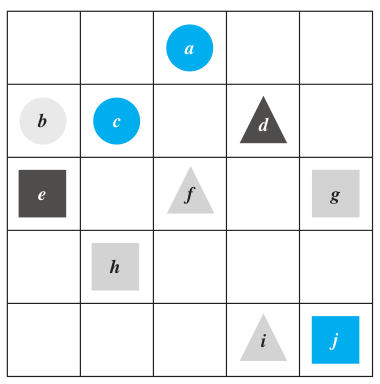
\includegraphics[scale=0.4]{../images/3.3.1.png}
\end{figure}

{\bf \color{cyan} The statements in exercises $5-8$ refer to the Tarski world given in Figure 3.3.1 (repeated above). Explain why each is true.}

\subsection{Exercise 5}
For every circle $x$ there is a square $y$ such that $x$ and $y$ have the same color.

\begin{proof}

\end{proof}

\subsection{Exercise 6}
For every square $x$ there is a circle $y$ such that $x$ and $y$ have different colors and $y$ is above $x$.

\begin{proof}

\end{proof}

\subsection{Exercise 7}
There is a triangle $x$ such that for every square $y$, $x$ is above $y$.

\begin{proof}

\end{proof}

\subsection{Exercise 8}
There is a triangle $x$ such that for every circle $y$, $y$ is above $x$.

\begin{proof}

\end{proof}

\subsection{Exercise 9}
Let $D = E = \{-2, -1, 0, 1, 2\}$. Explain why the following statements are true.

\subsubsection{(a)}
$\fa x$ in $D$, $\te y$ in $E$ such that $x + y = 0$.

\begin{proof}

\end{proof}

\subsubsection{(b)}
$\te x$ in $D$ such that $\fa y$ in $E$, $x + y = y$.

\begin{proof}

\end{proof}

\subsection{Exercise 10}
This exercise refers to Example 3.3.3. Determine whether each of the following statements is true or false.

\subsubsection{(a)}
$\fa$ student $S$, $\te$ a dessert $D$ such that $S$ chose $D$.

\begin{proof}

\end{proof}

\subsubsection{(b)}
$\fa$ student $S$, $\te$ a salad $T$ such that $S$ chose $T$.

\begin{proof}

\end{proof}

\subsubsection{(c)}
$\te$ a dessert $D$ such that $\fa$ student $S$, $S$ chose $D$.

\begin{proof}

\end{proof}

\subsubsection{(d)}
$\te$ a beverage $B$ such that $\fa$ student $D$, $D$ chose $B$.

\begin{proof}

\end{proof}

\subsubsection{(e)}
$\te$ an item $I$ such that $\fa$ student $S$, $S$ did not choose $I$.

\begin{proof}

\end{proof}

\subsubsection{(f)}
$\te$ a station $Z$ such that $\fa$ student $S$, $\te$ an item $I$ such that $S$ chose $I$ from $Z$.

\begin{proof}

\end{proof}

\subsection{Exercise 11}
Let $S$ be the set of students at your school, let $M$ be the set of movies that have ever been released, and let $V(s, m)$ be “student $s$ has seen movie $m$.” Rewrite each of the following statements without using the symbol $\fa$, the symbol $\te$, or variables.

\subsubsection{(a)}
$\te s \in S$ such that $V(s$, Casablanca).

\begin{proof}

\end{proof}

\subsubsection{(b)}
$\fa s \in S$, $V(s$, Star Wars).

\begin{proof}

\end{proof}

\subsubsection{(c)}
$\fa s \in S$, $\te m \in M$ such that $V(s, m)$.

\begin{proof}

\end{proof}

\subsubsection{(d)}
$\te m \in M$ such that $\fa s \in S$, $V(s, m)$.

\begin{proof}

\end{proof}

\subsubsection{(e)}
$\te s \in S$, $\te t \in S$, and $\te m \in M$ such that $s \neq t$ and $V(s, m) \wedge V(t, m)$.

\begin{proof}

\end{proof}

\subsubsection{(f)}
$\te s \in S$ and $\te t \in S$ such that $s \neq t$ and $\fa m \in M$, $V(s, m) \to V(t, m)$.

\begin{proof}

\end{proof}

\subsection{Exercise 12}
Let $D = E = \{-2, -1, 0, 1, 2\}$. Write negations for each of the following statements and determine which is true, the given statement or its negation.

\subsubsection{(a)}
$\fa x$ in $D$, $\te y$ in $E$ such that $x + y = 1$.

\begin{proof}

\end{proof}

\subsubsection{(b)}
$\te x$ in $D$ such that $\fa y$ in $E$, $x + y = -y$.

\begin{proof}

\end{proof}

\subsubsection{(c)}
$\fa x$ in $D$, $\te y$ in $E$ such that $xy \geq y$.

\begin{proof}

\end{proof}

\subsubsection{(d)}
$\te x$ in $D$ such that $\fa y$ in $E$, $x \leq y$.

\begin{proof}

\end{proof}

{\bf \color{cyan} In each of $13-19$, (a) rewrite the statement in English without using the symbol $\fa$ or $\te$ or variables and expressing your answer as simply as possible, and (b) write a negation for the statement.}

\subsection{Exercise 13}
$\fa$ color $C$, $\te$ an animal $A$ such that $A$ is colored $C$.

\begin{proof}

\end{proof}

\subsection{Exercise 14}
$\te$ a book $b$ such that $\fa$ person $p$, $p$ has read $b$.

\begin{proof}

\end{proof}

\subsection{Exercise 15}
$\fa$ odd integer $n$, $\te$ an integer $k$ such that $n = 2k + 1$.

\begin{proof}

\end{proof}

\subsection{Exercise 16}
$\te$ a real number $u$ such that $\fa$ real number $v$, $uv = v$.

\begin{proof}

\end{proof}

\subsection{Exercise 17}
$\fa r \in \Q$, $\te$ integers $a$ and $b$ such that $r = a/b$.

\begin{proof}

\end{proof}

\subsection{Exercise 18}
$\fa x \in \R$, $\te$ a real number $y$ such that $x + y = 0$.
\begin{proof}

\end{proof}

\subsection{Exercise 19}
$\te x \in \R$ such that for every real number $y$, $x + y = 0$.
\begin{proof}

\end{proof}

\subsection{Exercise 20}
\begin{figure}[ht!]
\centering
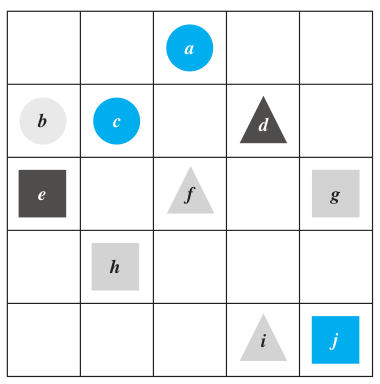
\includegraphics[scale=0.4]{../images/3.3.1.png}
\end{figure}

Recall that reversing the order of the quantifiers in a statement with two different quantifiers may change the truth value of the statement, but it does not necessarily do so. All the statements in the pairs below refer to the Tarski world of Figure 3.3.1. In each pair, the order of the quantifiers is reversed but everything else is the same. For each pair, determine whether the statements have the same or opposite truth values. Justify your answers.

\subsubsection{(a)}
(1) For every square $y$ there is a triangle $x$ such that $x$ and $y$ have different colors.

(2) There is a triangle $x$ such that for every square $y$, $x$ and $y$ have different colors.

\begin{proof}

\end{proof}

\subsubsection{(b)}
(1) For every circle $y$ there is a square $x$ such that $x$ and $y$ have the same color.

(2) There is a square $x$ such that for every circle $y$, $x$ and $y$ have the same color.

\begin{proof}

\end{proof}

\subsection{Exercise 21}
For each of the following equations, determine which of the following statements are true:

(1) For every real number $x$, there exists a real number $y$ such that the equation is true.

(2) There exists a real number $x$, such that for every real number $y$, the equation is true.

Note that it is possible for both statements to be true or for both to be false.

\subsubsection{(a)}
$2x + y = 7$

\begin{proof}

\end{proof}

\subsubsection{(b)}
$y + x = x + y$

\begin{proof}

\end{proof}

\subsubsection{(c)}
$x^2 - 2xy + y^2 = 0$

\begin{proof}

\end{proof}

\subsubsection{(d)}
$(x - 5)(y - 1) = 0$

\begin{proof}

\end{proof}

\subsubsection{(e)}
$x^2 + y^2 = -1$

\begin{proof}

\end{proof}

{\bf \color{cyan} In 22 and 23, rewrite each statement without using variables or the symbol $\fa$ or $\te$. Indicate whether the statement is true or false.}

\subsection{Exercise 22}
\subsubsection{(a)}
$\fa$ real number $x$, $\te$ a real number $y$ such that $x + y = 0$.

\begin{proof}

\end{proof}

\subsubsection{(b)}
$\te$ a real number $y$ such that $\fa$ real number $x$, $x + y = 0$.

\begin{proof}

\end{proof}

\subsection{Exercise 23}
\subsubsection{(a)}
$\fa$ nonzero real number $r$, $\te$ a real number $s$ such that $rs = 1$.

\begin{proof}

\end{proof}

\subsubsection{(b)}
$\te$ a real number $r$ such that $\fa$ nonzero real number $s$, $rs = 1$.

\begin{proof}

\end{proof}

\subsection{Exercise 24}
Use the laws for negating universal and existential statements to derive the following rules:

\subsubsection{(a)}
$\sim(\fa x \in D(\fa y \in E(P(x, y)))) \equiv \te x \in D(\te y \in E({\sim P(x, y)}))$

\begin{proof}

\end{proof}

\subsubsection{(b)}
$\sim(\te x \in D(\te y \in E(P(x, y)))) \equiv \fa x \in D(\fa y \in E({\sim P(x, y)}))$

\begin{proof}

\end{proof}

\begin{figure}[ht!]
\centering
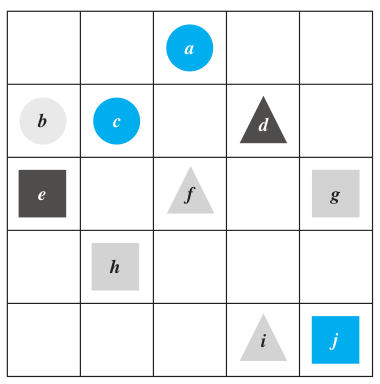
\includegraphics[scale=0.4]{../images/3.3.1.png}
\end{figure}

{\bf \color{cyan} Each statement in $25-28$ refers to the Tarski world of Figure 3.3.1 (repeated above). For each, (a) determine whether the statement is true or false and justify your answer, and (b) write a negation for the statement (referring, if you wish, to the result in exercise 24).}

\subsection{Exercise 25}
$\fa$ circle $x$ and $\fa$ square $y$, $x$ is above $y$.

\begin{proof}

\end{proof}

\subsection{Exercise 26}
$\fa$ circle $x$ and $\fa$ triangle $y$, $x$ is above $y$.

\begin{proof}

\end{proof}

\subsection{Exercise 27}
$\te$ a circle $x$ and $\te$ a square $y$ such that $x$ is above $y$ and $x$ and $y$ have different colors.

\begin{proof}

\end{proof}

\subsection{Exercise 28}
$\te$ a triangle $x$ and $\te$ a square $y$ such that $x$ is above $y$ and $x$ and $y$ have the same color.

\begin{proof}

\end{proof}

{\bf \color{cyan} For each of the statements in 29 and 30, (a) write a new statement by interchanging the symbols $\fa$ and $\te$, and (b) state which is true: the given statement, the version with interchanged quantifiers, neither, or both.}

\subsection{Exercise 29}
$\fa x \in \R, \te y \in \R$ such that $x < y$.

\begin{proof}

\end{proof}

\subsection{Exercise 30}
$\te x \in \R$ such that $\fa y \in \R^-$ (the set of negative real numbers), $x > y$.

\begin{proof}

\end{proof}

\subsection{Exercise 31}
Consider the statement “Everybody is older than somebody.” Rewrite this statement in the form “$\fa$ people $x$, $\te$ \fbl.”

\begin{proof}

\end{proof}

\subsection{Exercise 32}
Consider the statement “Somebody is older than everybody.” Rewrite this statement in the form “$\te$ a person $x$ such that $\fa$ \fbl.”

\begin{proof}

\end{proof}

{\bf \color{cyan} In $33-39$, (a) rewrite the statement formally using quantifiers and variables, and (b) write a negation for the statement.}

\subsection{Exercise 33}
Everybody loves somebody.

\begin{proof}

\end{proof}

\subsection{Exercise 34}
Somebody loves everybody.

\begin{proof}

\end{proof}

\subsection{Exercise 35}
Everybody trusts somebody.

\begin{proof}

\end{proof}

\subsection{Exercise 36}
Somebody trusts everybody.

\begin{proof}

\end{proof}

\subsection{Exercise 37}
Any even integer equals twice some integer.

\begin{proof}

\end{proof}

\subsection{Exercise 38}
Every action has an equal and opposite reaction.

\begin{proof}

\end{proof}

\subsection{Exercise 39}
There is a program that gives the correct answer to every question that is posed to it.

\begin{proof}

\end{proof}

\subsection{Exercise 40}
In informal speech most sentences of the form “There is \fbl every \fbl” are intended to be understood as meaning “$\fa$ \fbl $\te$ \fbl,” even though the existential quantifier {\it there is} comes before the universal quantifier {\it every}. Note that this interpretation applies to the following well-known sentences. Rewrite them using quantifiers and variables.

\subsubsection{(a)}
There is a sucker born every minute.

\begin{proof}

\end{proof}

\subsubsection{(b)}
There is a time for every purpose under heaven.

\begin{proof}

\end{proof}

\subsection{Exercise 41}
Indicate which of the following statements are true and which are false. Justify your answers as best you can.

\subsubsection{(a)}
$\fa x \in \Z^+ \te y \in \Z^+$ such that $x = y + 1$.

\begin{proof}

\end{proof}

\subsubsection{(b)}
$\fa x \in \Z \te y \in \Z$ such that $x = y + 1$.

\begin{proof}

\end{proof}

\subsubsection{(c)}
$\te x \in \R$ such that $\fa y \in \R$, $x = y + 1$.

\begin{proof}

\end{proof}

\subsubsection{(d)}
$\fa x \in \R^+ \te y \in \R^+$ such that $xy = 1$.

\begin{proof}

\end{proof}

\subsubsection{(e)}
$\fa x \in \R \te y \in \R$ such that $xy = 1$.

\begin{proof}

\end{proof}

\subsubsection{(f)}
$\te x \in \R$ such that $\fa y \in \R$, $x + y = y$.

\begin{proof}

\end{proof}

\subsubsection{(g)}
$\te x \in \R$ such that $\fa y \in \R$, $y < x$.

\begin{proof}

\end{proof}

\subsubsection{(h)}
$\te x \in \R^+$ such that $\fa y \in \R^+$, $x \leq y$.

\begin{proof}

\end{proof}

\subsection{Exercise 42}
Write the negation of the definition of limit of a sequence given in Example 3.3.7.

\begin{proof}

\end{proof}

\subsection{Exercise 43}
The following is the definition for $\lim_{x \to a} f(x) = L$:

For every real number $\epsilon > 0$, there exists a real number $\delta > 0$ such that for every real number $x$, if $a - \delta < x < a + \delta$ and $x \neq a$ then 
$$
L - \epsilon < f(x) < L + \epsilon
$$

Write what it means for $\lim_{x \to a} f(x) \neq L$. In other words, write the negation of the definition.

\begin{proof}

\end{proof}

\subsection{Exercise 44}
The notation $\te$! stands for the words “there exists a unique.” Thus, for instance, “$\te$! $x$ such that $x$ is prime and $x$ is even” means that there is one and only one even prime number. Which of the following statements are true and which are false? Explain.

\subsubsection{(a)}
$\te$! real number $x$ such that $\fa$ real number $y$, $xy = y$.

\begin{proof}

\end{proof}

\subsubsection{(b)}
$\te$! integer $x$ such that $1/x$ is an integer.

\begin{proof}

\end{proof}

\subsubsection{(c)}
$\fa$ real number $x$, $\te$! real number $y$ such that $x + y = 0$.

\begin{proof}

\end{proof}

\subsection{Exercise 45}
Suppose that $P(x)$ is a predicate and $D$ is the domain of $x$. Rewrite the statement “$\te$! $x \in D$ such that $P(x)$” without using the symbol $\te$!. (See exercise 44 for the meaning of $\te$!.)

\begin{proof}

\end{proof}

\begin{figure}[ht!]
\centering
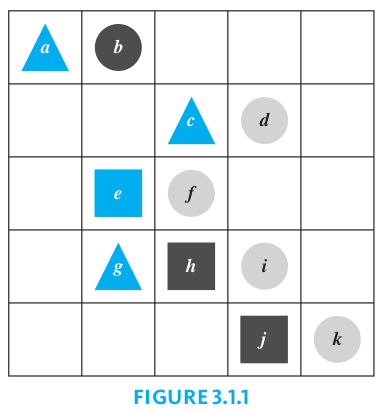
\includegraphics[scale=0.4]{../images/3.1.1.png}
\end{figure}

{\bf \color{cyan} In $46-54$, refer to the Tarski world given in Figure 3.1.1, which is shown again here for reference. the domains of all variables consist of all the objects in the Tarski world. For each statement, (a) indicate whether the statement is true or false and justify your answer, (b) write the given statement using the formal logical notation illustrated in example 3.3.10, and (c) write a negation for the given statement using the formal logical notation of example 3.3.10.}

\subsection{Exercise 46}
There is a triangle $x$ such that for every square $y$, $x$ is above $y$.

\begin{proof}

\end{proof}

\subsection{Exercise 47}
There is a triangle $x$ such that for every circle $y$, $x$ is above $y$.

\begin{proof}

\end{proof}

\subsection{Exercise 48}
For every circle $x$, there is a square $y$ such that $y$ is to the right of $x$.

\begin{proof}

\end{proof}

\subsection{Exercise 49}
For every object $x$, if $x$ is a circle then there is a square $y$ such that $y$ has the same color as $x$.

\begin{proof}

\end{proof}

\subsection{Exercise 50}
For every object $x$, if $x$ is a triangle then there is a square $y$ such that $y$ is below $x$.

\begin{proof}

\end{proof}

\subsection{Exercise 51}
There is a square $x$ such that for every triangle $y$, if $y$ is above $x$ then $y$ has the same color as $x$.

\begin{proof}

\end{proof}

\subsection{Exercise 52}
For every circle $x$ and for every triangle $y$, $x$ is to the right of $y$.

\begin{proof}

\end{proof}

\subsection{Exercise 53}
There is a circle $x$ and there is a square $y$ such that $x$ and $y$ have the same color.

\begin{proof}

\end{proof}

\subsection{Exercise 54}
There is a circle $x$ and there is a triangle $y$ such that $x$ has the same color as $y$.

\begin{proof}

\end{proof}

{\bf \color{cyan} Let $P(x)$ and $Q(x)$ be predicates and suppose $D$ is the domain of $x$. In $55-58$, for the statement forms in each pair, determine whether (a) they have the same truth value for every choice of $P(x), Q(x)$, and $D$, or (b) there is a choice of $P(x), Q(x)$, and $D$ for which they have opposite truth values.}

\subsection{Exercise 55}
$\fa x \in D, (P(x) \wedge Q(x))$, and $(\fa x \in D, P(x)) \wedge (\fa x \in D, Q(x))$

\begin{proof}

\end{proof}

\subsection{Exercise 56}
$\te x \in D, (P(x) \wedge Q(x))$, and $(\te x \in D, P(x)) \wedge (\te x \in D, Q(x))$

\begin{proof}

\end{proof}

\subsection{Exercise 57}
$\fa x \in D, (P(x) \vee Q(x))$, and $(\fa x \in D, P(x)) \vee (\fa x \in D, Q(x))$

\begin{proof}

\end{proof}

\subsection{Exercise 58}
$\te x \in D, (P(x) \vee Q(x))$, and $(\te x \in D, P(x)) \vee (\te x \in D, Q(x))$

\begin{proof}

\end{proof}

{\bf \color{cyan} In $59-61$, find the answers Prolog would give if the following questions were added to the program given in example 3.3.11.}

\subsection{Exercise 59}

\subsubsection{(a)}
?isabove$(b_1, w_1)$

\begin{proof}

\end{proof}

\subsubsection{(b)}
?color($X$, white)

\begin{proof}

\end{proof}

\subsubsection{(c)}
?isabove$(X, b_3)$

\begin{proof}

\end{proof}

\subsection{Exercise 60}

\subsubsection{(a)}
?isabove$(w_1, g)$

\begin{proof}

\end{proof}

\subsubsection{(b)}
?color$(w_2$, blue)

\begin{proof}

\end{proof}

\subsubsection{(c)}
?isabove$(X, b_1)$

\begin{proof}

\end{proof}

\subsection{Exercise 61}

\subsubsection{(a)}
?isabove$(w_2, b_3)$

\begin{proof}

\end{proof}

\subsubsection{(b)}
?color($X$, gray)

\begin{proof}

\end{proof}

\subsubsection{(c)}
?isabove$(g, X)$

\begin{proof}

\end{proof}

\section{Exercise Set 3.4}

\subsection{Exercise 1}
Let the following law of algebra be the first statement of an argument: For all real numbers $a$ and $b$, 
$$
(a + b)^2 = a^2 + 2ab + b^2. 
$$
Suppose each of the following statements is, in turn, the second statement of the argument. Use universal instantiation or universal modus ponens to write the conclusion that follows in each case.

\subsubsection{(a)}
$a = x$ and $b = y$ are particular real numbers.

\begin{proof}

\end{proof}

\subsubsection{(b)}
$a = f_i$ and $b = f_j$ are particular real numbers.

\begin{proof}

\end{proof}

\subsubsection{(c)}
$a = 3u$ and $b = 5v$ are particular real numbers.

\begin{proof}

\end{proof}

\subsubsection{(d)}
$a = g(r)$ and $b = g(s)$ are particular real numbers.

\begin{proof}

\end{proof}

\subsubsection{(e)}
$a = \log(t_1)$ and $b = \log(t_2)$ are particular real numbers.

\begin{proof}

\end{proof}

{\bf \color{cyan} Use universal instantiation or universal modus ponens to fill in valid conclusions for the arguments in $2-4$.}

\subsection{Exercise 2}
If an integer $n$ equals $2\cdot k$ and $k$ is an integer, then $n$ is even.

0 equals $2\cdot 0$ and 0 is an integer.

$\therefore$ \fbl

\begin{proof}

\end{proof}

\subsection{Exercise 3}
For all real numbers $a, b, c$, and $d$, if $b \neq 0$ and $d \neq 0$ then $a/b + c/d = (ad + bc)/bd$.

$a = 2, b = 3, c = 4$, and $d = 5$ are particular real numbers such that $b = 0$ and $d \neq 0$.

$\therefore$ \fbl

\begin{proof}

\end{proof}

\subsection{Exercise 4}
$\fa$ real numbers $r, a$, and $b$, if $r$ is positive, then $(r^a)^b = r^{ab}$.

$r = 3, a = 1/2$, and $b = 6$ are particular real numbers such that $r$ is positive.

$\therefore$ \fbl

\begin{proof}

\end{proof}

{\bf \color{cyan} Use universal modus tollens to fill in valid conclusions for the arguments in 5 and 6.}

\subsection{Exercise 5}
All irrational numbers are real numbers.

$1/0$ is not a real number.

$\therefore$ \fbl

\begin{proof}

\end{proof}

\subsection{Exercise 6}
If a computer program is correct, then compilation of the program does not produce error messages.

Compilation of this program produces error messages.

$\therefore$ \fbl

\begin{proof}

\end{proof}

{\bf \color{cyan} Some of the arguments in 7–18 are valid by universal modus ponens or universal modus tollens; others are invalid and exhibit the converse or the inverse error. State which are valid and which are invalid. Justify your answers.}

\subsection{Exercise 7}
All healthy people eat an apple a day.

Keisha eats an apple a day.

$\therefore$ Keisha is a healthy person.

\begin{proof}

\end{proof}

\subsection{Exercise 8}
All freshmen must take a writing course.

Caroline is a freshman.

$\therefore$ Caroline must take a writing course.

\begin{proof}

\end{proof}

\subsection{Exercise 9}
If a graph has no edges, then it has a vertex of degree zero.

This graph has at least one edge.

$\therefore$ This graph does not have a vertex of degree zero.

\begin{proof}

\end{proof}

\subsection{Exercise 10}
If a product of two numbers is 0, then at least one of the numbers is 0.

For a particular number $x$, neither $(2x + 1)$ nor $(x - 7)$ equals 0.

$\therefore$ The product $(2x + 1)(x - 7)$ is not 0.

\begin{proof}

\end{proof}

\subsection{Exercise 11}
All cheaters sit in the back row. 

Monty sits in the back row.

$\therefore$ Monty is a cheater.

\begin{proof}

\end{proof}

\subsection{Exercise 12}
If an 8-bit two’s complement represents a positive integer, then the 8-bit two’s complement starts with a 0.

The 8-bit two’s complement for this integer does not start with a 0.

$\therefore$ This integer is not positive.

\begin{proof}

\end{proof}

\subsection{Exercise 13}
For every student $x$, if $x$ studies discrete mathematics, then $x$ is good at logic.

Tarik studies discrete mathematics.

$\therefore$ Tarik is good at logic.

\begin{proof}

\end{proof}

\subsection{Exercise 14}
If compilation of a computer program produces error messages, then the program is not correct.

Compilation of this program does not produce error messages.

$\therefore$ This program is correct.

\begin{proof}

\end{proof}

\subsection{Exercise 15}
Any sum of two rational numbers is rational.

The sum $r + s$ is rational.

$\therefore$ The numbers $r$ and $s$ are both rational.

\begin{proof}

\end{proof}

\subsection{Exercise 16}
If a number is even, then twice that number is even.

The number $2n$ is even, for a particular number $n$.

$\therefore$ The particular number $n$ is even.

\begin{proof}

\end{proof}

\subsection{Exercise 17}
If an infinite series converges, then the terms go to 0.

The terms of the infinite series $\dps \sum_{n = 1}^{\infty} \frac{1}{n}$ go to 0.

$\therefore$ The infinite series $\dps \sum_{n = 1}^{\infty} \frac{1}{n}$ converges.

\begin{proof}

\end{proof}

\subsection{Exercise 18}
If an infinite series converges, then its terms go to 0.

The terms of the infinite series $\dps \sum_{n = 1}^{\infty} \frac{n}{n+1}$ do not go to 0.

$\therefore$ The infinite series $\dps \sum_{n = 1}^{\infty} \frac{n}{n+1}$ does not converge.

\begin{proof}

\end{proof}

\subsection{Exercise 19}
Rewrite the statement “No good cars are cheap” in the form “$\fa x$, if $P(x)$ then $\sim Q(x)$.” Indicate whether each of the following arguments is valid or invalid, and justify your answers.

\subsubsection{(a)}
No good car is cheap.

A Rimbaud is a good car.

$\therefore$ A Rimbaud is not cheap.

\begin{proof}

\end{proof}

\subsubsection{(b)}
No good car is cheap.

A Simbaru is not cheap.

$\therefore$ A Simbaru is a good car.

\begin{proof}

\end{proof}

\subsubsection{(c)}
No good car is cheap.

A VX Roadster is cheap.

$\therefore$ A VX Roadster is not good.

\begin{proof}

\end{proof}

\subsubsection{(d)}
No good car is cheap.

An Omnex is not a good car.

$\therefore$ An Omnex is cheap.

\begin{proof}

\end{proof}

\subsection{Exercise 20}

\subsubsection{(a)}
Use a diagram to show that the following argument can have true premises and a false conclusion.

All dogs are carnivorous.

Aaron is not a dog.

$\therefore$ Aaron is not carnivorous.

\begin{proof}

\end{proof}

\subsubsection{(b)}
What can you conclude about the validity or invalidity of the following argument form? Explain how the result from part (a) leads to this conclusion.

$\fa x$, if $P(x)$ then $Q(x)$.

$\sim P(a)$ for a particular $a$.

$\therefore$ $\sim Q(a)$.

\begin{proof}

\end{proof}

{\bf \color{cyan} Indicate whether the arguments in $21-27$ are valid or invalid. Support your answers by drawing diagrams.}

\subsection{Exercise 21}
All people are mice.

All mice are mortal.

$\therefore$ All people are mortal.

\begin{proof}

\end{proof}

\subsection{Exercise 22}
All discrete mathematics students can tell a valid argument from an invalid one.

All thoughtful people can tell a valid argument from an invalid one.

$\therefore$ All discrete mathematics students are thoughtful.

\begin{proof}

\end{proof}

\subsection{Exercise 23}
All teachers occasionally make mistakes.

No gods ever make mistakes.

$\therefore$ No teachers are gods.

\begin{proof}

\end{proof}

\subsection{Exercise 24}
No vegetarians eat meat.

All vegans are vegetarian.

$\therefore$ No vegans eat meat.

\begin{proof}

\end{proof}

\subsection{Exercise 25}
No college cafeteria food is good.

No good food is wasted.

$\therefore$ No college cafeteria food is wasted.

\begin{proof}

\end{proof}

\subsection{Exercise 26}
All polynomial functions are differentiable.

All differentiable functions are continuous.

$\therefore$ All polynomial functions are continuous.

\begin{proof}

\end{proof}

\subsection{Exercise 27}
Nothing intelligible ever puzzles me.

Logic puzzles me.

$\therefore$ Logic is unintelligible.

\begin{proof}

\end{proof}

{\bf \color{cyan} In exercises $28-32$, reorder the premises in each of the arguments to show that the conclusion follows as a valid consequence from the premises. It may be helpful to rewrite the statements in if-then form and replace some of them by their contrapositives. exercises $28-30$ refer to the kinds of Tarski worlds discussed in examples 3.1.13 and 3.3.1. exercises 31 and 32 are adapted from Symbolic Logic by Lewis Carroll.}

\subsection{Exercise 28}
1. Every object that is to the right of all the blue objects is above all the triangles.

2. If an object is a circle, then it is to the right of all the blue objects.

3. If an object is not a circle, then it is not gray. 

$\therefore$ All the gray objects are above all the triangles.

\begin{proof}

\end{proof}

\subsection{Exercise 29}
1. All the objects that are to the right of all the triangles are above all the circles.

2. If an object is not above all the black objects, then it is not a square.

3. All the objects that are above all the black objects are to the right of all the triangles.

$\therefore$ All the squares are above all the circles.

\begin{proof}

\end{proof}

\subsection{Exercise 30}
1. If an object is above all the triangles, then it is above all the blue objects.

2. If an object is not above all the gray objects, then it is not a square.

3. Every black object is a square.

4. Every object that is above all the gray objects is above all the triangles.

$\therefore$ If an object is black, then it is above all the
blue objects.

\begin{proof}

\end{proof}

\subsection{Exercise 31}
1. I trust every animal that belongs to me.

2. Dogs gnaw bones.

3. I admit no animals into my study unless they will beg when told to do so.

4. All the animals in the yard are mine.

5. I admit every animal that I trust into my study.

6. The only animals that are really willing to beg when told to do so are dogs.

$\therefore$ All the animals in the yard gnaw bones.

\begin{proof}

\end{proof}

\subsection{Exercise 32}
1. When I work a logic example without grumbling, you may be sure it is one I understand.

2. The arguments in these examples are not arranged in regular order like the ones I am used to.

3. No easy examples make my head ache.

4. I can’t understand examples if the arguments are not arranged in regular order like the ones I am used to.

5. I never grumble at an example unless it gives me a headache.

$\therefore$ These examples are not easy.

\begin{proof}

\end{proof}

{\bf \color{cyan} In 33 and 34 a single conclusion follows when all the given premises are taken into consideration, but it is difficult to see because the premises are jumbled up. reorder the premises to make it clear that a conclusion follows logically, and state the valid conclusion that can be drawn.
(It may be helpful to rewrite some of the statements in if-then form and to replace some statements by their contrapositives.)}

\subsection{Exercise 33}
33. 1. No birds except ostriches are at least 9 feet tall.
2. There are no birds in this aviary that belong to
anyone but me.
3. No ostrich lives on mince pies.
4. I have no birds less than 9 feet high.

\begin{proof}

\end{proof}

\subsection{Exercise 34}
1. All writers who understand human nature are clever.

2. No one is a true poet unless he can stir the human heart.

3. Shakespeare wrote Hamlet.

4. No writer who does not understand human nature can stir the human heart.

5. None but a true poet could have written Hamlet.

\begin{proof}

\end{proof}

\subsection{Exercise 35}
Derive the validity of universal modus tollens from the validity of universal instantiation and modus tollens.

\begin{proof}

\end{proof}

\subsection{Exercise 36}
Derive the validity of universal form of part (a) of the elimination rule from the validity of universal instantiation and the valid argument called elimination in Section 2.3.

\begin{proof}

\end{proof}

\end{document}
